\documentclass[conference]{IEEEtran}
\usepackage{amsmath,amssymb,amsfonts}
\usepackage{ucs}
\usepackage[utf8x]{inputenc}
\usepackage[english]{babel}
\usepackage[nottoc]{tocbibind}
\usepackage[left=2.5cm,right=2.5cm,top=2.5cm,bottom=2.5cm,]{geometry}
\usepackage{graphicx}
\usepackage{nameref}
\usepackage[hidelinks]{hyperref}
\usepackage{sidecap}
\usepackage{wrapfig}
\usepackage[bottom,hang]{footmisc} 
\usepackage{acronym}
\usepackage{multirow}
\usepackage{color}
\usepackage{capt-of}
\usepackage{array,			%better tables
			tabularx,			    %instead of tabular*             
			booktabs,			%tables for good publications
}
\usepackage{afterpage,hyperref} 
\usepackage{listings}
\usepackage{subfigure}


\begin{document}
\title{Seminar on Privacy in Ubiquitous Computing}

\author{\IEEEauthorblockN{Mehmed Mustafa}
\IEEEauthorblockA{\textit{Institute of Computer Science} \\
\textit{University of Göttingen}\\
mehmed.mustafa@stud.uni-goettingen.de}
\and
\IEEEauthorblockN{Chris Warin}
\IEEEauthorblockA{\textit{Institute of Computer Science} \\
\textit{University of Göttingen}\\
chris.warin@stud.uni-goettingen.de
}
}

\maketitle

\begin{abstract}
This document is a model and instructions for \LaTeX.
This and the IEEEtran.cls file define the components of your paper [title, text, heads, etc.]. *CRITICAL: Do Not Use Symbols, Special Characters, Footnotes, 
or Math in Paper Title or Abstract.
\end{abstract}

\begin{IEEEkeywords}
privacy, bystander, privacy enhancing technology
\end{IEEEkeywords}

\section{Introduction}
Today's society is filled with technological devices that are capable of gathering data from people, such as smartphones \cite{lu2017privacy}, surveillance cameras \cite{denning2014situ}, \ac{AR} devices \cite{shu2016cardea} or \ac{IoT} devices \cite{lu2017privacy}. Although these devices been causing a number of concerns regarding the privacy of users, another topic---that is less publicly discussed, but as important---is the privacy of bystanders, i.e. the people that are around users using these devices, and of which personal information can be collected without their knowledge or consent. 

A common real-life example could be a person taking a picture in a busy street, where the faces of bystanders are recognizable. The picture can later be posted on social media, and neither the posting or the taken picture have been made with the knowledge nor consent of the bystanders \cite{shu2016cardea}. The data that are collected from bystanders can come from different mediums (i.e. pictures, videos, audio), and can be of different nature (i.e. face, voice, location). This results in pervasiveness in bystanders' privacy and touches several domains, namely economical, social, legal, and technological. 

In the past, several attempts have been made in order to ensure the privacy of bystanders; technological attempts (e.g. gaussian blur, pixelisation \cite{dufaux2010framework}), as well as partial solutions to avoid privacy issues (e.g. forbidding the use of cameras in certain places\cite{shu2016cardea}). However, these have been proven either inefficient~\cite{dufaux2010framework} or insufficient~\cite{shu2016cardea}. 

This report focuses on the different technologies that address the pervasiveness in the privacy of bystanders. Section~\ref{BystandersPrivacy} lists different real-life examples of bystanders' privacy being compromised. Section~\ref{Technologies} goes over different technologies that ensure different aspects of the privacy of bystanders. Section~\ref{Limitations} describes the current limitations and challenges that these technologies are facing, whether they are technological or not. Finally, section~\ref{Conclusion} concludes this report.

\section{Bystanders’ privacy pervasiveness}\label{BystandersPrivacy}
Give real-life examples and why they are problematic.
\subsection{Videos and images}
Surveillance cameras, smartphone photos/videos in the street capturing bystanders
\subsection{Audio}
Google Home / Amazon Alexa in a household: other members are also listened
\subsection{Location}
Pervasive location information in apps (e.g. French StopCovid app recenses more contacts’ location information than announced)
\subsection{Others}
IoT, see example in 2.b

\section{Technologies for ensuring the privacy of bystanders}\label{Technologies}

\subsection{PriSurv System}
Video surveillance systems are necessary for a safe and secure community, which explains why they are widely deployed. However, high deployment rate of these systems in public places leads to privacy invasion of the objects being recorded. Solution of this problem is a challenging task because privacy and security should be balanced appropriately and when possible in real-time.
There are several other studies on privacy based on video surveillance. Two studies proposed image processing methods in order to protect the privacy of objects \cite{cavallaro2005}\cite{kitahara2004}. In some other studies the privacy protection of objects depends either on the authority of objects or observers \cite{jehan2005}\cite{senior2005}. Privacy information can be embedded by using digital watermarking technology in a such way that only predefined authorized viewers will have access to it \cite{zhang2005}. However, these solutions are not flexible enough, because the sense of privacy of different objects is not considered. For example, object A may want his or her privacy to be protected from observer A, but not from observer B. Some objects may not want a privacy protection at all. 
PriSurv system \cite{chinomi2008PriSurv} can adaptively protect privacy of objects and disclosure their visual information according to the privacy policies of the different objects. PriSurv is a video surveillance system, which is defined by visual abstraction and protects the privacy of objects appearing within a video depending who observes the video. Closeness between objects and observers determines the privacy policies to be used. 

\begin{figure}[t]
\centerline{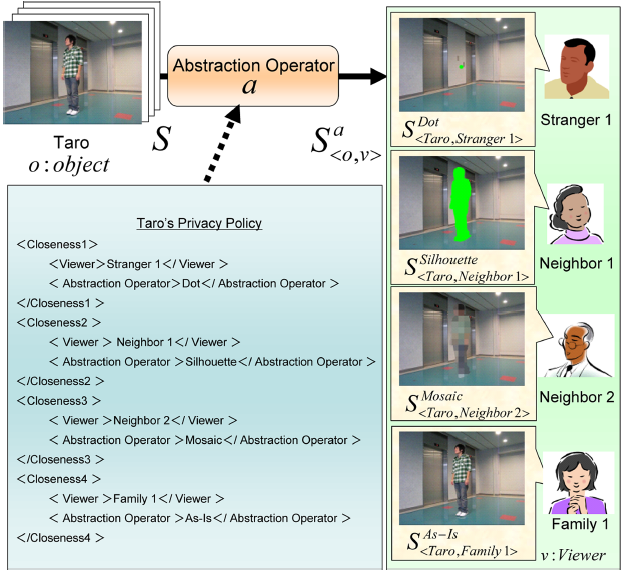
\includegraphics[width=.5\textwidth]{img//prisurv_simple_demo.png}}
\caption{PriSurv simple run case \cite{chinomi2008PriSurv}.}
\label{fig:prisurv}
\end{figure}

\subsubsection{Simple run case}
Figure~\ref{fig:prisurv} is an example run case of PriSurv, which shows how visual abstraction is used in order to protect the privacy of an object appearing within an image. Let o, a, v and S denote an object, an abstraction operator, a viewer and an original image, respectively. In the example, “Taro” is the object which appears within the original image and is monitored by “Stranger 1”, “Neighbor 1”, “Neighbor 2” and “Family 1” which are the different viewers. Since the closeness between the object and viewers is different, different abstraction operators are used for hiding the visual information of the object. In the example, these operators are “Dot”, “Silhouette”, “Mosaic” and “As-Is”, just 4 out of 12 possible. Each viewer then receives a privacy protected version of the original image which is denoted by $S_{<o, v>}^a$. A simplified version of Taro’s privacy policy, which is a part of the abstraction operator, is also available to give better understanding how the closeness is defined. 

\begin{figure}[t]
\centerline{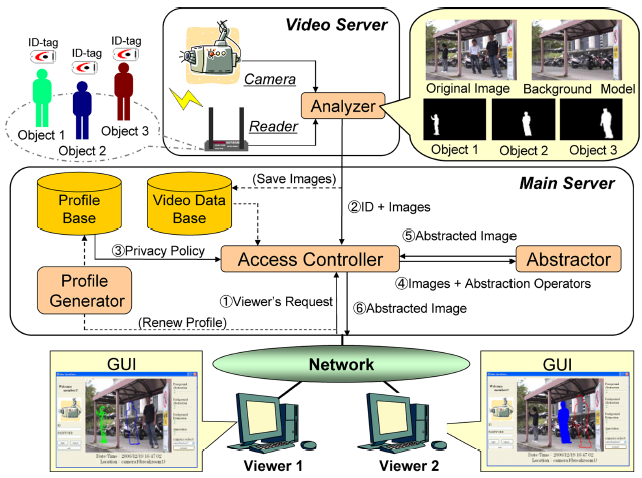
\includegraphics[width=.5\textwidth]{img//prisurv_arch.png}}
\caption{PriSurv system overview \cite{chinomi2008PriSurv}.}
\label{fig:prisurv2}
\end{figure}

\subsubsection{System overview}
Figure~\ref{fig:prisurv2} shows the architecture of the PriSurv system. It consists of three main parts: Video Server, Main Server and Network. It also has six different components: Analyzer, Profile Generator, Profile Base, Access Controller, Abstractor and Video Data Base. Analyzer, which is a part of the video server, is responsible for identifying different objects. Each identifiable object must have own \ac{RFID}-tag. The surveillance area is divided into smaller N x N areas and the location area of each \ac{RFID}-tag is determined by an \ac{RFID}-reader. Each object inside the original image is extracted and then identified separately by comparing the obtained visual data with the binary images of each object. Profile Generator is used for setting up privacy policies for different members of the system. Each member's personal information such as name, age, gender and address and privacy policy stored securely inside the Profile Base. Profile Generator is also responsible for converting data taken from the GUI to \ac{XML} based syntax. The profile of each member can be updated only by them and other members have no access to this data. Access Controller determines what is the closeness relationship between a requesting viewer and an object to be monitored by reading \ac{XML} based privacy policies of the object stored inside the Profile Base. Once the types of abstraction operators are extracted, Access Controller sends them to the Abstractor. Abstractor is a processor for images which does visual abstraction by using abstraction operators. Video Data Base stores past video data and makes it available to viewers after appropriate visual abstractions are performed. 



\subsection{Sharing of Multi-Subject and Interdependent Data}
Reference \cite{olteanu2018consensual}

\subsection{Cardea Framework}
Reference \cite{shu2016cardea}

\begin{figure}[t]
\centerline{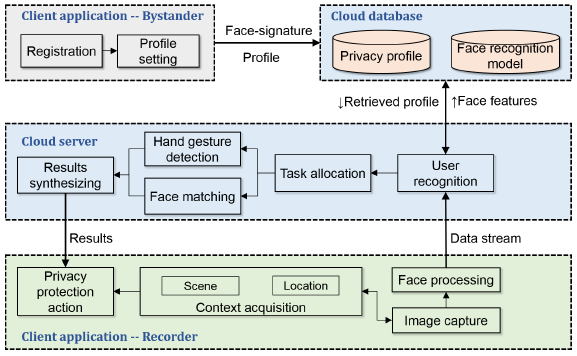
\includegraphics[width=.5\textwidth]{img/cardea_overview_diagram.png}}
\caption{Cardea framework overview \cite{shu2016cardea}.}
\label{fig:cardea}
\end{figure}

\subsection{Others - More specific Audio or Location based technologies should be found}


\section{Limitations and challenges of privacy ensuring technologies}\label{Limitations}
\subsection{Cardea (user contribution)}
Willingly putting your personal data on a cloud to avoid having your privacy invaded by others can be seen as counter productive
\subsection{Example 2}
\subsection{Example 3}
\subsection{(optionally) Ideas that could fix these limitations}

\section{Conclusion}\label{Conclusion}


\begin{table}[htbp]
\caption{Table Type Styles}
\begin{center}
\begin{tabular}{|c|c|c|c|}
\hline
\textbf{Table}&\multicolumn{3}{|c|}{\textbf{Table Column Head}} \\
\cline{2-4} 
\textbf{Head} & \textbf{\textit{Table column subhead}}& \textbf{\textit{Subhead}}& \textbf{\textit{Subhead}} \\
\hline
copy& More table copy$^{\mathrm{a}}$& &  \\
\hline
\multicolumn{4}{l}{$^{\mathrm{a}}$Sample of a Table footnote.}
\end{tabular}
\label{tab1}
\end{center}
\end{table}

\section*{References}

Please number citations consecutively within brackets \cite{shu2016cardea}. The 
sentence punctuation follows the bracket \cite{dufaux2010framework}. Refer simply to the reference 
number, as in \cite{denning2014situ}---do not use ``Ref. \cite{denning2014situ}'' or ``reference \cite{denning2014situ}'' except at 
the beginning of a sentence: ``Reference \cite{lu2017privacy} was the first $\ldots$''

Number footnotes separately in superscripts.\cite{chinomi2008PriSurv} Place the actual footnote at 
the bottom of the column in which it was cited. Do not put footnotes in the 
abstract or reference list. Use letters for table footnotes.

Unless there are six authors or more give all authors' names; do not use 
``et al.''. Papers that have not been published, even if they have been 
submitted for publication, should be cited as ``unpublished'' \cite{lu2017privacy}. Papers 
that have been accepted for publication should be cited as ``in press'' \cite{olteanu2018consensual}. 
Capitalize only the first word in a paper title, except for proper nouns and 
element symbols.\cite{sen2016ipic}

For papers published in translation journals, please give the English 
citation first, followed by the original foreign-language citation \cite{olteanu2018consensual}.

\section*{Abbreviations and Acronyms}
\addcontentsline{toc}{section}{Abbreviations and Acronyms}
\begin{acronym}[Bash]
\acro{IoT} {\textit{Internet of Things}}
\acro{AR} {\textit{Augmented Reality}}
\acro{RFID} {\textit{Radio-frequency identification}}
\acro{XML} {\textit{Extensible Markup Language}}
\end{acronym}

\bibliographystyle{ieeetr}
{\footnotesize
\bibliography{literature_list}}

\end{document}